\section{Benchmark and Protocol}
\label{sec:benchmark}

\begin{figure*}[t]
  \centering
  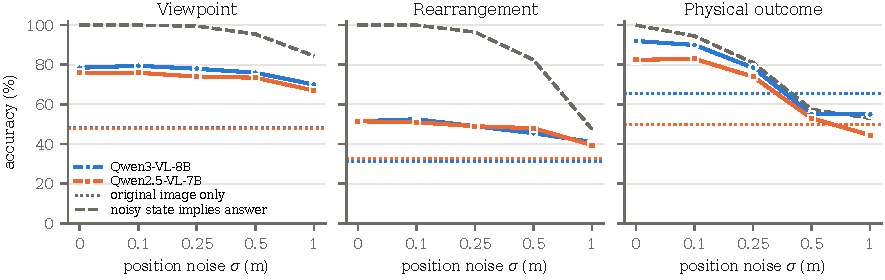
\includegraphics[width=\linewidth]{figs/noise.pdf}
  \caption{\textbf{Accuracy with a degraded oracle} (Qwen models). Solid: accuracy when the imagined state is rendered from object positions perturbed with Gaussian noise $\sigma$. Dotted: the same model with the original image only. Gray dashed: how often the perturbed state still implies the correct answer.}
  \label{fig:noise}
\end{figure*}

\paragraph{Scenes and rendering.} Scenes contain 4--6 spheres, cubes and cylinders on a floor, each with a unique color, rendered at $448{\times}448$ pixels with a 40$^\circ$ field of view by a small ray tracer with shadows. Every scene is an exact 3D description, so any changed state can be rendered without approximation.

\paragraph{Tasks.} We generate 200 questions for each of three tasks (\cref{fig:teaser}). \emph{Viewpoint}: after walking a quarter or half way around the scene, is object A to the left or right of object B? \emph{Rearrangement}: after A trades places with B, which object is closest to A? \emph{Physical outcome}: will a stack of 3--4 offset blocks stay standing when released? Stability follows from the center of mass of each sub-stack relative to its support. Answers are computed from geometry, with margins that exclude borderline cases (a screen-space gap of at least 8\% of the image width; a nearest/second-nearest distance ratio of at least 1.4; a center of mass at least 8\,cm from any tipping edge).

\paragraph{Shortcut controls.} Binary answers are balanced by construction. For viewpoint, half the questions have an answer that differs from the one in the current view, so answering from the current view scores 50\%. For rearrangement, the answer is never the swap partner nor the target's nearest neighbor before the swap.

\paragraph{Conditions.} The model always sees the original image and the question, and answers with one option. \textbf{Img.}: nothing else. \textbf{Text}: it first describes the changed scene in words. \textbf{Oracle}: a second image shows the exact imagined state. \textbf{Misl.}: the second image shows a plausible imagined state with a different answer (another viewpoint, another swap, the opposite outcome). \textbf{Unrel.}: the second image is the oracle of a different question of the same task. \textbf{Oracle alone}: the imagined state replaces the original image, with its own wording (supplementary). \textbf{Own}: the model first lists every object and its floor position as JSON; we apply the change described in the question and render the result as the second image. All two-image conditions use identical wording, so the model cannot tell them apart from the prompt.

\paragraph{Models.} Qwen3-VL-8B-Instruct~\cite{qwen2025qwen3vl}, Qwen2.5-VL-7B-Instruct~\cite{bai2025qwen25vl} and InternVL3-8B~\cite{zhu2025internvl3}, all with 4-bit NF4 weights, Qwen3-VL-32B-Instruct (4-bit, without Text and Own), and Qwen2.5-VL-3B-Instruct in bf16 as a smaller reference; greedy decoding. Because of its length, ``Text'' is run on 100 questions per task (Qwen2.5-VL-7B: all 200; Qwen3-VL-8B: 200 on rearrangement). We report accuracy, and compare conditions on the same questions with exact McNemar tests, Holm-corrected over all comparisons.
